\documentclass[10pt,conference]{IEEEtran}

\usepackage{lmodern}
\usepackage{amssymb,amsmath}
\usepackage{ifxetex,ifluatex}
\usepackage{multirow}
\usepackage{booktabs}
\usepackage{fixltx2e} % provides \textsubscript

\usepackage[backend=bibtex,style=numeric]{biblatex}
\bibliography{bibliography.bib}

\ifnum 0\ifxetex 1\fi\ifluatex 1\fi=0 % if pdftex
  \usepackage[T1]{fontenc}
  \usepackage[utf8]{inputenc}
\else % if luatex or xelatex
  \ifxetex
    \usepackage{mathspec}
  \else
    \usepackage{fontspec}
  \fi
  \defaultfontfeatures{Ligatures=TeX,Scale=MatchLowercase}
\fi
% use upquote if available, for straight quotes in verbatim environments
\IfFileExists{upquote.sty}{\usepackage{upquote}}{}
% use microtype if available
\IfFileExists{microtype.sty}{%
\usepackage{microtype}
\UseMicrotypeSet[protrusion]{basicmath} % disable protrusion for tt fonts
}{}
\usepackage{hyperref}
\PassOptionsToPackage{usenames,dvipsnames}{color} % color is loaded by hyperref
\hypersetup{unicode=true,
            pdftitle={CS229 Project Milestone},
            pdfauthor={Honghao Qiu},
            colorlinks=true,
            linkcolor=black,
            citecolor=Blue,
            urlcolor=Blue,
            breaklinks=true}
\urlstyle{same}  % don't use monospace font for urls
\usepackage{graphicx,grffile}
\makeatletter
\def\maxwidth{\ifdim\Gin@nat@width>\linewidth\linewidth\else\Gin@nat@width\fi}
\def\maxheight{\ifdim\Gin@nat@height>\textheight\textheight\else\Gin@nat@height\fi}
\makeatother
% Scale images if necessary, so that they will not overflow the page
% margins by default, and it is still possible to overwrite the defaults
% using explicit options in \includegraphics[width, height, ...]{}
\setkeys{Gin}{width=\maxwidth,height=\maxheight,keepaspectratio}
\IfFileExists{parskip.sty}{%
\usepackage{parskip}
}{% else
\setlength{\parindent}{0pt}
\setlength{\parskip}{6pt plus 2pt minus 1pt}
}
\setlength{\emergencystretch}{3em}  % prevent overfull lines
\providecommand{\tightlist}{%
  \setlength{\itemsep}{0pt}\setlength{\parskip}{0pt}}
\setcounter{secnumdepth}{5}
% Redefines (sub)paragraphs to behave more like sections
\ifx\paragraph\undefined\else
\let\oldparagraph\paragraph
\renewcommand{\paragraph}[1]{\oldparagraph{#1}\mbox{}}
\fi
\ifx\subparagraph\undefined\else
\let\oldsubparagraph\subparagraph
\renewcommand{\subparagraph}[1]{\oldsubparagraph{#1}\mbox{}}
\fi
\usepackage{subfig}
\AtBeginDocument{%
\renewcommand*\figurename{Figure}
\renewcommand*\tablename{Table}
}
\AtBeginDocument{%
\renewcommand*\listfigurename{List of Figures}
\renewcommand*\listtablename{List of Tables}
}
\usepackage{float}
\floatstyle{ruled}
\makeatletter
\@ifundefined{c@chapter}{\newfloat{codelisting}{h}{lop}}{\newfloat{codelisting}{h}{lop}[chapter]}
\makeatother
\floatname{codelisting}{Listing}
\newcommand*\listoflistings{\listof{codelisting}{List of Listings}}

\title{Multiview Human Synthesis From a Singleview}
\author{Si Wen (06246679), Tiancong Zhou (06247022), Honghao Qiu (06246258)\\
\texttt{\{wensi, longztc, honq\}{@}stanford.edu}}

% Begin custom, non-pandoc commands.

\newcommand{\latexonlyrule}{\rule}

% End custom, non-pandoc commands.

\begin{document}
\maketitle

\newcommand{\R}{\mathbb{R}}
\newcommand{\eqnset}[1]{\left.\mbox{$#1$}\quad\quad\right\rbrace}
\newcommand{\tr}{\text{tr}\;}
\renewcommand{\th}{\theta}
\newcommand{\toi}{^{(i)}}

%comments

\textbf{Abstract --  }
\textbf{We use deep generative models to synthesize multiview images given a single view. The generation process is done in two stages: in the first stage, we train a variational auto-encoder (VAE) \autocite{kingma2013auto} to synthesize a new view of the input image; in the second stage, we use a generative adversarial network (GAN) \autocite{goodfellow2014generative} to generate details on the output of the first stage. We evaluate our results using both qualitative and quantitative methods. One potential application is generating multiview images for e-Commerce products.}


\section{Introduction} 
Multiview synthesis has been a long standing problem in computer vision. Traditionally, this problem had been attempted using geometry-based approaches. That is, a 3D model is first reconstructed from the input image, and the novel view is generated from that 3D model. However, with recent progress in deep learning, more and more people have attempted to synthesize novel views directly use deep neural networks \autocite{yim2015rotating, tatarchenko2016multi, zhao2017multi, zhou2016view, huang2017beyond, kueflerdeep, park2017transformation}, and have achieved great results.

Our project limits the scope of the multiview synthesis problem to human images, with a focus on the clothing items in these images. Given the recent progress in deep generative models and their amazing results on image synthesize and style transfer \autocite{oord2016pixel, isola2016image, zhu2017unpaired, karras2017progressive}, we try to tackle this problem using similar approaches. Our goal is to synthesize images of a particular person from any view given a single input view. If successful, this could enable many useful applications in fashion/E-Commerce websites and in the field of photo/video edition and content generation. For example, in Amazon cloth stores we can help provide 360-degree rotation view for customers given a single front-view image taken for the model.

To achieve this goal, we use images of people with different dress in different angles as input data, with both real world multiview fashion dataset from MVC \autocite{liu2016mvc} and synthetic human images rendered in 360-degree views. Then we use deep neural networks to generate output images from the inputs in a two-stage process. First, the input image (human body in a specific angle) and the value of target angle (e.g. 90 degree) are fed into a VAE to generate a coarse image output in the target angle, and then this coarse image along with the original input image are both fed into a GAN to generate a fine image in the target angle.

Figure 1 further illustrates the idea of this process with a specific example.

\begin{figure}[htbp]
\centering
\includegraphics{Model.PNG}
\caption{Condition input image is firstly inputed into VAE to generate coarse view image for target angle, then it is inputed into GAN to generate fine view image for target angle.}
\end{figure}


\section{Related Work}
In recent years, there have been numerous attempts to solve subsets of this problem. 

On one hand, some previous research attempt to generate full human body image for some specific angles given the front view. For example, Zhao et al [2] proposed a VAE+GAN model to synthesize the side and back view of a person given the frontal view. This approach has the strength of combining the ability of VAE to find global appearance/outline and the ability of GAN to fill in fine details. This approach inspires us to try a very similar model pipeline. However, there are several limitations in their work: 1. in their paper, their model inputs the target image into VAE for generating coarse image output, where we want to get rid of this input, 2. due to the limitation of available data, their model only generates side and back view image outputs, and cannot be extended to output images for any target angle, 3. their work mainly focuses on the person’s clothing, and the resulting image contains poorly synthesized face. Our work would try to overcome these limitations.

On the other hand, some other researches work on generating specific areas of human, such as faces, hands, etc. instead of full human body, and still, due to the limitation of available data, the synthesis outputs are typically in limited views such as front/side/back view. For example, Huang et al [3] proposed a method to provide photorealistic synthesis of the frontal views of a person’s face given a side view. We try to leverage some of their loss functions that are helpful for face synthesis and include them into our method when we generate multiview images of an entire person.

There are some other related works for object rotation [6,8] (such as car/chair), and 3d model generation based on multiview images [3,5,6]. Some of their work [] has reached pretty good results for generating 360-degree synthesis by using [TODO: MODEL], but this task is relatively less difficult compared to multiview human and fashion synthesis since the target object output typically contains less details and simpler texture to be generated. 

\section{Dataset and Features}
Solving this problem requires large amount of training data for the network to learn the latent representation. We use a combination of real world datasets and synthetic datasets. We used a combination of MVC datasets (160,000 real images) and 80,000 synthetic images (360-degrees views). Image data are labeled with the associated angles for the view (e.g. 60 degree). Due to this relatively large dataset, we use around 1\% images for testing and the rest of data for training.

Since the currently available real world views are rather limited and often only have frontal, back, and side views, we try to overcome this limitation by using 360-degree synthetic images generated from 3D modeling softwares. We also notice that some past usage of synthetic data on vision problems has shown promising results [2,5,6].

Our 360-degree human view dataset (about 100,000 full-body human images in 360-degree views) is generated by the following approach:
\renewcommand{\labelenumi}{\roman{enumi}}
 \begin{enumerate}
   \item Create 3D character models in Adobe Fuse. Adobe Fuse provides plenty of hairstyles, faces, cloth and shoes to combine and create 3D characters;
   \item Export the model as .obj file;
   \item Import the obj file into Blender. (Blender is a 3D graphics software that could be programmed and rendered to generate 360-degree views);
   \item Render and generate front view;
   \item Rotate the 3D character model by 1 degree clockwise, render and generate new view from that degree;
   \item Repeat step 5 and 6 until generating views for all 360 degrees.   
 \end{enumerate}

Figure 2 contains some examples of synthetic images we generated.

\begin{figure}[htbp]
\centering
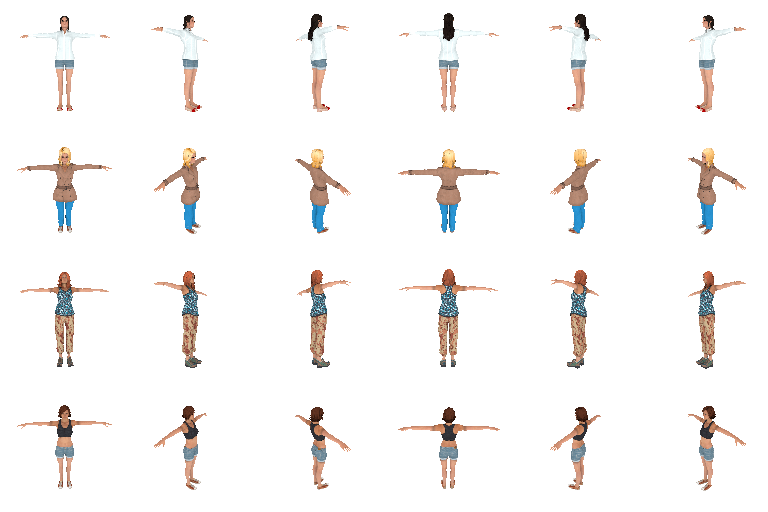
\includegraphics{data.png}
\caption{Synthetic Multiview Human Image Samples}
\end{figure}



\section{Methods}

\subsection{Overview}

We tackle this problem using deep generative models. We divide our pipeline into two stages: the first stage consists of an input image, a target angle (0 to 360 degrees), and a conditional VAE. The encoder transforms the input image into a latent variable, concatenate it with the target angle, and passes them through the decoder. The decoded image should resemble the input image in the target angle, with noticeable artifact (e.g. blurry, sometimes with incorrect colors). The second stage consists of the original input image, output of the first stage (coarse image), and a conditional GAN. Both images are fed into a hierarchical feature extractor to obtain their latent representations. These latent representations are then concatenated and fed into a generator to obtain the final output. The generator is able to extract low level patterns from the original input image and generate a new image that conforms to the structure of the coarse image with patterns from the original input image.

\subsection{Variational Auto-Encoder (VAE)}

Similar to GAN taught in the class, Variational Auto-Encoder is a generative deep neural network, instead of learning through an adversarial process, it tries to approximate the data distribution directly using KL divergence and a reconstruction loss. Because of this, it is easier to train than a GAN, and is able to consistently generate the global appearance of the input image in a target view. However, since it assumes the data comes from a normal distribution, it often produces blurry results. 

In the first stage of our pipeline, the VAE encodes the input image, concatenates it with the target angle (scalar value in [0, 360]), and feeds them through the decoder to produce an image in the target view.


\subsection{Generative Adversarial Network (GAN)}

Since VAE result primarily captures global appearance but lacks details, we hope to use a generative network to fill in these details for making fine image, and this is what GAN is capable of doing. At the same time, the conditional conditions we introduced to the GAN makes it more stable during training and thus making the generated final result with much higher quality.

As is shown in the second stage of our pipeline in figure 3, we feed the input image and the output from VAE through a Siamese network to produce the final fine image in the target view, and is trained adversarially.

\subsection{Pipeline Overview}
We combines variants of the Generative Adversarial Network (GAN) [1] to solve this problem. GAN is a generative approach that learns a distribution to represent the training data. We can then generate new images sampled from that distribution, conditioned on the input image and the desired angles. Figure 3 illustrates our pipeline.

\begin{figure*}[htbp]
\centering
\includegraphics{Picture2.png}
\caption{Pipeline Overview}
\end{figure*}

As is shown in Zhao et al paper [VariGan, 2], GAN is good at filling rich details of the synthesized image but less capable of capturing global appearance and rough outlines for human/clothings, and on the other hand, VAE [7] is more capable of finding global appearance with less detailed details, therefore, GAN and VAE are good complements of each other for image synthesis. Our model follows the following two-step approach to achieve image synthesis: 1) firstly use VAE to model coarse global appearance (outline/structure of the image), 2) then use variants of GAN to model refined details of the person and get fine synthesized images of full human body in multiviews. Compared to Zhao's model, we did not input the target image into VAE, but instead only input conditional image and the target angle to VAE model. Another improvement we are making is, with our synthetic data for human body from all angles, we target at outputting all 360-degree multiview human synthesis from a given view of any angle. This is achieved by changing the angle degree input in the VAE model during training process according to the label of target output image (i.e. the target angle). 


\subsection{Network Architecture}
\textbf{VAE Architecture} 
We use 6 convolution layers in the VAE encoder to down sample input image and use a fully connected layer to transform it into a 1024-dimension representation. Then, the latent variable is passed into the 6 layer convolutional layer decoder along with embedded target view angle to generate a $128\times128\times3$ image.

\textbf{GAN Architecture} 
The generator for fine image is a Siamese network which contains two weights-sharing encoders to process conditional image and coarse image output by VAE. We use a similar architecture to VAE here, where 6 layers convolution layers are used to find the 1024-dimension representation of the input images, and then it is up-sampled by the decoder (also a 6 layer CNN) to generate the $128\times128\times3$ fine image output.

\subsection{Objective (Loss) Function}
We mainly use the following loss functions (with penalty factor assigned to each loss and calculating the combined loss as objective loss function):

\begin{itemize}
\item Adversarial loss:\\
Our adversarial loss is defined as:
$$ E_{I_v \sim p_{data(I_v)}}[log D(I_v)] + E_{z \sim p(z)}[log (1- D(I_v, G(z, I_v)))], $$
here $I_v$ stands for Image given a Viewpoint, D is the discriminator and G is the generator to be trained simultaneously. This is closely adapted from [1].

\item VAE loss:\\
As is shown in Bowman et al's work [11], we are also using the standard VAE loss term, which is defined as the sum of KL-divergence loss and a reconstruction loss term:
$$ L(\theta;x)= -KL(q_\theta(z|x)||p(z))+E_{q_\theta(z|x)}[log(p_\theta(x|z))] $$

\item Pixel to pixel loss:\\
One potential reason why VariGAN approach has a poor performance on head synthesis might be only adversarial loss being used in GAN's objective. Inspired by Huang et al's work [3], we try to model face generation better by using pixel to pixel comparison loss, in this way face features would be better captured since incorrectly predicted faces are penalized with additional loss (more details are discussed in Objective Function section).

The pixel-wise loss can be expressed as [3]:
$$ \frac{1}{L \times H} \sum_{x=1}^L \sum_{y=1}^H |\hat{I}_{x,y}- I_{x,y}|, $$
where L stands for Length (number of pixels in row-wise), and H stands for Height (number of pixels in column-wise). $\hat{I}_{x,y}$ is the predicted pixel of the image and $I_{x,y}$ is the corresponding pixel in GT.

\item Regularization term in loss function:\\
We use adaptive L2 regularization on the discriminator to penalize large weights and mitigate over-fitting. As is shown in [1], this is helpful when discriminator is too strong for the generator and the regularization term can be decreased when generator catches up with the discriminator.

\end{itemize}


\subsection{Implementation Details}

We implemented the VAE from scratch, and gradually 

\begin{figure}[htbp]
\centering
\includegraphics{experiments.png}
\caption{Row 1-4: output of VAEs with (1) fully-connected layers only with insufficient amount of  hidden neurons (2) fully-connected layers only with sufficient hidden neurons (3) convolutional layers with insufficient amount of filters (4) convolutional layers with sufficient amount of filters. }
\end{figure}

We attempted to implement a GAN from scratch. However, 

\section{Experimentation Results}

We use both quantitative and qualitative measures to assess the result of our work. 
There are a number of 

Figure 5 summarizes the image outputs by this VAE+GAN model on MVC and our synthetic dataset.

\begin{figure*}[htbp]
\centering
\includegraphics{PICTURE4.png}
\caption{//TODO: change to image output summarize graph}
\end{figure*}

\subsection{Qualitative results}

\begin{figure*}[htbp]
\centering
\includegraphics[width=50mm]{samples.png}
\caption{Sample images trained and tested using synthetic images. Left to right: input image, output from cVAE, output from cGAN, our from our model, ground truth.}
\end{figure*}

For quantitative evaluation methods, we use the Structural Similarity Index (SSIM), the Inception Score (IS), and Root Mean Square Errors (RMSE) to compare the generated fine image output to target image, as a judgment for our model quality.

\begin{itemize}
\item SSIM: Structural Similarity []:
$$SSIM(I_x,I_y)=\frac{(2\mu_x \mu_y + c_1)(2\sigma_{xy}+c_2)}{(\mu_x^2+\mu_y^2 +c_1)(\sigma_x^2+\sigma_y^2+c_2)}$$

\item IS: Inception Score []:
$$IS(I_x,I_y)=exp(E_{I_x}D_{KL(p(y|I_x)||p(y))})$$
where $I_x,I_y$ are generated image and GT image respectively, and y is the label (the input angle in our model).

\end{itemize}

For model comparison, we experimented the following 3 models on MVC and our synthetic dataset respectively, and compare the SSIM, IS, RMSE outputs:

1. Using only VAE

2. Using only GAN

3. Using our VAE+GAN pipeline

Figure 6 summarizes the result of our experimentations.
\begin{figure*}
  \includegraphics[width=\linewidth]{FigureTable.PNG}
  \caption{Experimental Results}
  \label{fig:boat1}
\end{figure*}

From the result metrics in the table, we can see that the following trends: 

1. SSIM obtained by our VAE+GAN approach is larger than that of obtained by using VAE or GAN alone, which means our generated output image is more similar to the ground truth; 

2. IS score for VAE+GAN is larger than that of using VAE only, but smaller than IS score using GAN only, this is expected since GAN model alone allows more variation in the output images. 

3. RMSE analysis shows that VAE+GAN RMSE is smaller than that of using VAE or GAN alone, this resonates with the result of SSIM and proves that our approach in general has better performance generating images closer to target. 

4. In general, our model performs better on synthetic data than on real world data, this is because synthetic data is smoother, contains less details, and has similar pose, so the generation is relatively easier. 


\section{Further Discussions and Future Work}

1. In general, our model works well on synthetic images, as there are less noise in the data (e.g. no background, unified pose, similar texture, etc.).

2. On MVC dataset, we achieved reasonably good result compared to other methods (see table above). Since VAE is capable of finding 
global appearance with less details, while GAN is good at filling rich details of the synthesized image but less capable of capturing 
global appearance and rough outlines for human/clothings, therefore, GAN and VAE complements each other well for image synthesis 
in our architecture. The coarse image generated by VAE captures global appearance, while GAN fills in details to make the fine image.

3. Our model does not perform well on face synthesis (compared to the body), since face contains more details and is harder to synthesize.

In the future, we plan to work on the followings:

1. Improve the GAN: we only used a simple conditional GAN with very little hyperparameter tuning. There is a number of recently published papers that shows various techniques to improve the quality and stability of GANs.

2. Improve face synthesis: our model currently handles face poorly since it contains a lot of noticeable details. It is important to be able to recreate these details in a convincing way for good result. 

3. Include background: our current dataset only contains images without any background. It is more difficult to synthesize views when the object of interest is not presented in isolation and we would like to tackle that problem in the future.


\section{Conclusion}
We aims at solving 360-degree full human body view synthesis problem by using our self-generated dataset and VAE+GAN modeling approach, while introducing some minor changes on modeling architecture and loss function compared with previous works [1,2,3].
Current preliminary results show some promising potential of our modeling approach. With the help of large volume self-generated human view data from 360 view angles, we hope we can solve the 360 degree full human body view synthesis problem and achieve state-of-art results.

\textbf{Teammate Contributions:}

Our teamwork break down:
\begin{itemize}
\item Si (Vincent) Wen: Vicent mainly works on modeling, including VAE and variants of GAN modeling, he also contributed to dataset generation (Fuse and MVC).
\item Tiancong Zhou: Tiancong mainly works on dataset generation (human viewed from 360 degrees in Blender), he also contributed to data processing.
\item Honghao Qiu: Honghao mainly works on modeling and reporting. He works on VAE+GAN modeling, super-resolution DC-GAN, and he is the main contributor to writing this report.
\end{itemize}

Our team target at equal contributions from three team members across data, modeling, and reporting.  In general, all our teammates have made equal contribution to this project so far. We hope to successfully finish the project with our collective efforts!


\printbibliography

\end{document}
